% !TEX encoding = UTF-8
% !TEX TS-program = pdflatex
% !TEX root = ../tesi.tex

%**************************************************************
\chapter{Progettazione e codifica}
\label{cap:progettazione-codifica}
%**************************************************************

\intro{
In questo capitolo vengono descritte le principali scelte progettuali, la struttura del database, la struttura del server e dell'applicativo client-side.}\\

%**************************************************************
%\section{Tecnologie e strumenti}
%\label{sec:tecnologie-strumenti}

%Di seguito viene data una panoramica delle tecnologie e strumenti utilizzati.

%\subsection*{Tecnologia 1}
%Descrizione Tecnologia 1.

%\subsection*{Tecnologia 2}
%Descrizione Tecnologia 2

%**************************************************************


\begin{figure}[h!]
\section{Database}
\label{sec:database}

Per gestire l'area di amministrazione degli utenti è stato costruito il database locale di amministrazione chiamato "data", appunto perché dovrà rappresenta tutti i dati amministrativi dell'utente, la gestione dell'associazione tra utenti b2b con quelli di telegram, le licenze degli utenti e tutta la gestione della tastiera telegram. La creazione e la  gestione della tastiera di telegram è automatizzata dalla tabella Keyboard, ovvero per creare un nuovo tasto associato ad una funzionalità, bisogna semplicemente scrivere sulla tabella Keyboard il nome del tasto, su quale riga si vuole posizionare e il nome del metodo che verrà chiamato quando si preme quel bottone. Questo sistema di gestione di tastiera è molto comodo per tenere una separazione tra i vari componenti che implementano una logica diversa. In questo modo è molto facile estendere l'applicativo con altre funzionalità modificando semplicemente una sola riga del database. 

   \begin{center}
     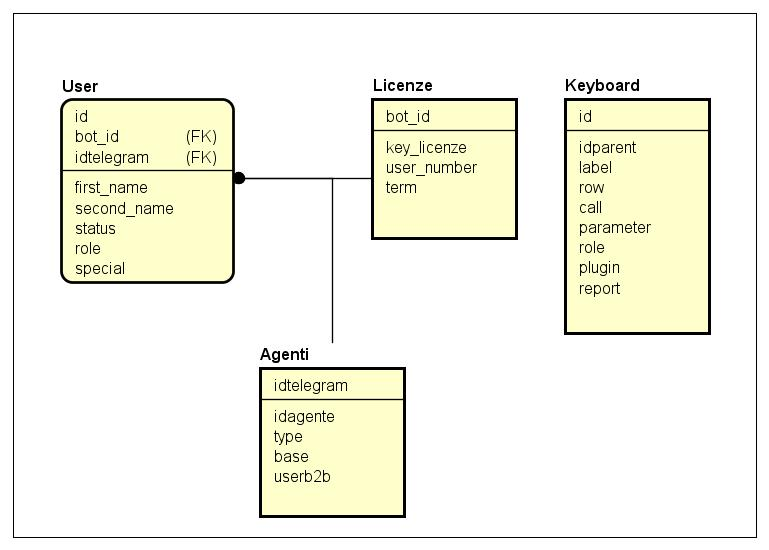
\includegraphics[scale=0.4]{diagrammi/database} 
    \caption{ER-Database }
    \end{center}

\subsection{Struttura}
In questa sottosezione verranno elencate tutte le tabelle che rappresentano la gestione dell'area amministrativa, spiegando il loro uso e funzionamento in modo da comprendere l'utilizzo che ne è stato fatto nel progetto per il salvataggio dei dati. \\
\end{figure}
\textbf{User} \\ 

In questa tabella vengono salvati i dati anagrafici dell'utente telegram,il suo ID identificativo univoco e il suo ruolo aziendale. \\

User ha i seguenti campi: \\ 
\begin{itemize}
\item \textbf{id:}  id univoco per identificare un univoco utente telegram;
\item \textbf{first\_name:} il nome dell'utente telegram;
\item \textbf{second\_name } il cognome dell'utente telegram;
\item \textbf{status:} lo status rappresenta se l'utente è abilitato "allow" oppure no, "deny";
\item \textbf{role:} role rappresenta il ruolo aziendale dell'utente;
\item \textbf{special:} special è un campo speciale utilizzato solo lato sviluppo per dare il massimo dei  permessi agli sviluppatore, utile in fase di testing;
\end{itemize}

\textbf{Agenti}\\

In questa tabella vengono salvati i dati riguardanti gli agenti, il loro Idtelegram, il loro tipo e la corrispondenza con il codice utente B2B.\\

La tabella Agenti presenta i seguenti campi:\\

\begin{itemize}
\item \textbf{id\_telegram:}  id univoco per identificare un univoco utente telegram;
\item \textbf{id\_agente:}  id univoco per identificare un agente;
\item \textbf{type:} rappresenta il tipo dell'agente;
\item \textbf{base:} rappresenta la base di appartenenza dell'agente;
\item \textbf{userb2b:} rappresenta il codice utente corrispondente in B2B;
\end{itemize}



\textbf{Licenze}
\\
In questa tabella vengono salvati i dati riguardanti le licenze con le loro scadenze per ciascun utente.\\

La tabella Licenze presenta i seguenti campi:

\begin{itemize}
\item \textbf{bot\_id:}  botid rappresenta l'ID univoco per identificare un utente telegram;
\item \textbf{key\_licenze:} rappresenta la chiave di licenza per gli utenti telegram;
\item \textbf{user\_number } rappresenta il numero massimo di account utilizzabili;
\item \textbf{term} rappresenta la data di scadenza della licenza;
\end{itemize}




\textbf{Keyboard}\\

In questa tabella vengono salvati i dati che riguardano la generazione della tastiera, la posizione e il nome del tasto.\\

La tabella Keyboard presenta i seguenti campi:\\

\begin{itemize}
\item \textbf{id:} id rappresenta l'ID associato al tasto univoco per identificare un utente telegram;
\item \textbf{id\_parent:} rappresenta la l'id del padre sul quale appendere il tasto;
\item \textbf{label } il campo label rappresenta l'etichetta del bottone;
\item \textbf{row } il campo row rappresenta il numero di riga dove si vuole aggiungere il tasto;
\item \textbf{call:} rappresenta la chiamata al metodo da effettuare quando si preme il bottone;
\item \textbf{parameter } parameter rappresenta i  parametri del metodo da chiamare
\item \textbf{role:} role rappresenta il ruolo dell'utente (admin oppure user);
\item \textbf{plugin } rappresenta il nome del plugin associato se c'è ne sono;
\item \textbf{report} rappresenta il nome del report;
\end{itemize}

\clearpage


\begin{figure}
\section{Back-end}
\label{sec:backend}
 \begin{center}
     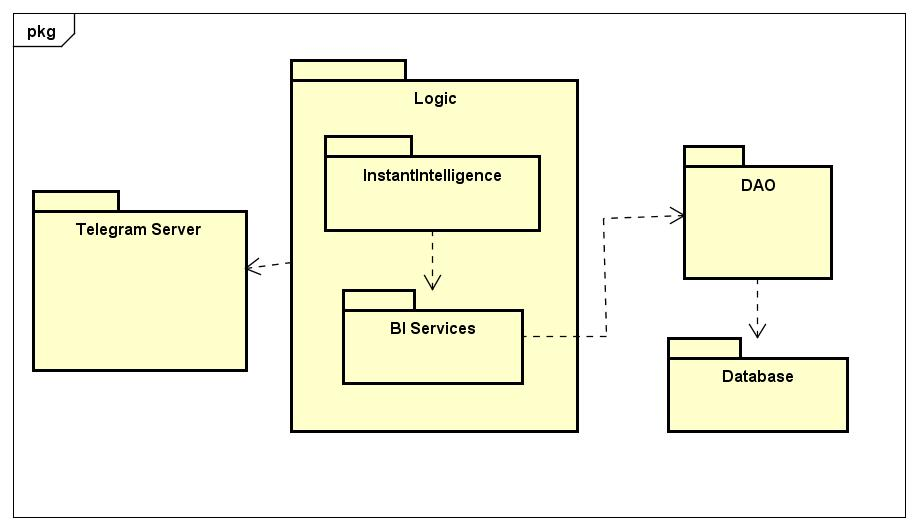
\includegraphics[scale=0.4]{diagrammi/Diagramm_backend} 
    \caption{Diagramma Back-end }
    \end{center}

\end{figure}  




\begin{figure}
\subsection{Server Telegram}
\label{sec:backend}
 \begin{center}
     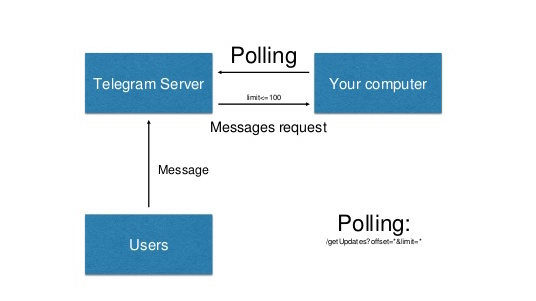
\includegraphics[scale=0.55]{diagrammi/polling} 
    \caption{Diagramm Polling }
    \end{center}

\end{figure}  






Nel progetto è stato implementato il metodo di long polling per le notifiche di telegram. Questo significa che ci si collega periodicamente al server telegram per aggiornarsi delle nuove notifiche. Come si vede nella prima figura, l'utente invia un messaggio ad un altro utente (in questo caso chiamato Your Computer). Il messaggio arriva al server telegram, il quale manda la richiesta al destinatario, dopodichè avviene il polling del messaggio verso il server. \\
Per la risposta invece il messaggio viene mandato prima al server telegram, successivamente viene mandato dal server all’utente desiderato.
\\Non possiamo dire nulla invece al riguardo del server telegram (il quale lo consideriamo come un Black-Box), poichè il codice sorgente del server telegram  non è disponibile ancora open source per il momento.


%


\subsection{InstantIntelligence}

Il package InstantIntelligence invece è la parte dove vengono elaborate le richieste dell'utente in base al tasto premuto. In questo package viene effettuato il controllo dell’autenticazione dell'utente, ovvero viene controllato se l’utente abbia una licenza valida oppure è la prima volta che sta accedendo e quindi sta chiedendo di essere abilitato.  Questo package si occupa anche della creazione e gestione della tastiera con i dati presi nel database Keyboard. Ogni richiesta fatta dall'utente, premendo un tasto oppure digitando un semplice comando passa per InstantIntelligence ed in base alla richiesta viene chiamato il relativo servizio BI, il quale si occuperà a sua volta di creare l'oggetto DAO corrispondente. \\\\

\subsubsection{Descrizione dei metodi più importanti}


\begin{itemize}
\item \textit{public void onUpdateReceived(Update update) :}  
questo metodo è il metodo che viene chiamato quando arriva un qualsiasi messaggio dall'utente telegram. Il parametro update invece è il contenuto del messaggio arrivato. I messaggi interessati nel nostro caso sono quelli che contengono una stringa come testo dato che il contenuto della stringa sarà fondamentale per chiamare successivamente il servizio giusto.

\item \textit{private boolean isWhiteListed(int id):}
il metodo isWhiteListed fà il controllo dell'utente se risulta registrato nella lista White dove sono memorizzati tutti gli utenti abilitati con una licenza. Il controllo viene effettuato sul parametro id dell'utente telegram. Se l'utente con codice id non fa parte della lisa White, viene mandato indietro un messaggio che avvisa l'utente di riprovare tra qualche minuto poichè si sta aspettando che un amministratore lo abiliti. 

\item \textit{private void handleIncomingMessage(Message message) :}
il metodo handleIncomingMessage è il gestore dei messaggi in arrivo e viene chiamato dopo il controllo del tipo di utente, ovvero se il metodo isWhiteListed ha ritornato true; 
handleIncomingMessage fà il paring sul contenuto del messaggio ed applica uno switch su  tutti i servizi da chiamare. Questo metodo ha il compito di costruire la tastiera iniziale se il "case" corrisponde al comando di "/start", altrimenti viene chiamato uno dei servizi, il quale prende la responsabilità di costruire la tastiera in base al comando ricevuto dal contenuto dell'oggetto Message.

	 \item \textit{private void onWelcomeMessage(String id, String firstName, ReplyKeyboardMarkup keyboardMarkup):} questo metodo contiene il messaggio iniziale di benvenuto e si occupa di caricare il menu principale da cui scegliere i vari processi. 

 \item \textit{private void onGetCommand(Message message, String queryResult):}
questo metodo gestisce tutti i comandi personalizzati e viene chiamato quando la query che si vuole fare risulta immediata e non necessita di un tasto nel menu.

 \item \textit{private void onGetReport(Message message, String call):}
onGetReport è il metodo che si occupa di inviare il report all’utente richiesto con la data e ora locale.

\item \textit{private static ReplyKeyboardMarkup getKeyboard(int idpadre):}
questo metodo si occupa di creare la tastiera corrente in base all'id padre rappresentato dalla tastiera appena nascosta quando è stato premuto un bottone. 

\item \textit{private static ReplyKeyboardMarkup getStartKeyboard():}
questo metodo costruisce la tastiera di start con i tasti predisposti in orizzontale.

\end{itemize}

\subsection{BI Services}

In questa sottosezione vengono descritti i servizi chiamati per creare e gestire i report. \\

\begin{itemize}

\item \textit{BDG\_Ordini\_Service:}Questo servizio si occupa di creare l'oggetto DAO che conterrà la lista degli ordini. Con un ciclo "for" si crea un unico oggetto di tipo stringa che rappresenta a secondo del DAO creato l'ordinato del giorno, l'ordinato di inizio mese oppure l'ordinato residuo. Il tipo di ritorno sarà una stringa poichè dovrà essere spedita al front-end come un messaggio di testo attraverso il metodo sendMessage(Message msg).

\item \textit{BDG\_Scadenze\_Service:}Questo servizio se occupa di creare e gestire le Scadenze che possono essere di tre tipi: Scadenze totali, Scaduto e Scadere. Anche questo servizio come BDG\_Ordini\_Service, in base alla richiesta dell'utente calcola e ritorna l'ammontare delle scadenze.

\item \textit{BDG\_Spedito\_Service:}BDG\_Spedito\_Service è uno dei tre servizi che si occupa di calcolare l'ammontare degli spediti che possono essere: Spedito oggi, Spedito ieri e Spedito questo mese. Questi tre servizi attualmente non fanno troppe operazione ma in futuro sono previsti calcoli più complessi.

\item \textit{BDG\_Disponibilità\_Service:}Questo servizio ha il compito di generare un documento con delle tabelle che contengono  la disponibilità degli articoli ordinati per codice articolo. BDG\_Disponibilità\_Service tiene conto della profilazione per codice agente.

\item \textit{BDG\_Inevasi\_Service:}Questo servizio genera il documento degli inevasi posizionando i dati in una tabella ordinati per numero di articolo. BDG\_Inevasi\_Service tiene conto della profilazione per codice agente.

\item \textit{BDG\_Scadenzario\_Service:}Questo servizio genera i documenti per lo scadenzario che possono essere di tre tipi: Scaduti, a scadere e insieme Scaduti/A scadere. BDG\_Scadenzario\_Service tiene conto della profilazione per codice agente.

\end{itemize}

\subsection{DAO}
Lo strato \gls{DAO} fondamentalmente ha una classe con relativi metodi che rappresenta
un'entità tabellare di un database e viene utilizzato per stratificare e isolare l'accesso
ad una tabella tramite query, che nel nostro caso sono costruite con una struttura Java
o interfacciandosi direttamente con il DAO. L'accesso al \gls{data-layer} da parte della
business-logic viene quindi controllato tramite DAO, creando un maggiore livello di
astrazione ed una più facile manutenibilità. I metodi del DAO con le rispettive query
verranno così richiamati dalle classi della business-logic.


\clearpage
\section{Front-end}

La parte Front-end di telegram è costituita principalmente dal menù principale che contiene i bottoni della tastiera, l'area di composizione del messaggio da inviare e l'area che visualizza la history della chat. In questa sezione si cerca di dare una panoramica generale di quelli che sono i componenti principali che compongono la tastiera interattiva dell'utente e i passi da seguire per poter portare a termine correttamente un operazione. Le figure saranno affiancate da una descrizione che illustra il funzionamento di vari componenti. 
Le operazioni che un utente può eseguire sono suddivisi in due blocchi: il primo contiene tutti i report disponibili e la loro gestione, il secondo blocco invece è accessibile solo dagli utenti amministratori e rappresenta la gestione dell'area amministrativa degli utenti generici. \\


\begin{figure}[h!]
\begin{center} \textbf{Menu principale} \end{center}
\begin{center}
    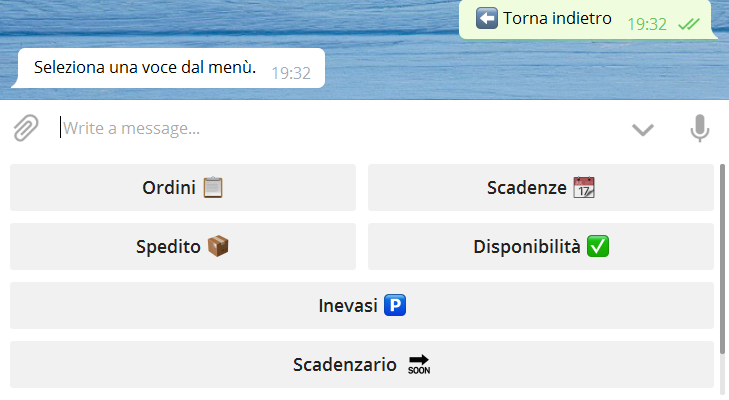
\includegraphics[scale=0.7]{screen/menu_principale} 
    \caption{Menu principale}
    \end{center}
Questa figura rappresenta il menu principale dove un utente generale può eseguire una delle operazioni disponibili nella tabella. Invece l'utente amministratore può accedere anche all'area amministrativa per la gestione delle licenze e l'associazione degli utenti. Per il bottone di Ordini, Scadenze e Spedizioni è presente l'ultimo livello dove l'utente può effettuare direttamente una richiesta di visualizzazione dell'ammontare (in euro) sul display. Per ciascun menù, all'ultima riga della tastiera è presente il tasto "Indietro"che permette di ritornare nel menù precedente. 
\end{figure}  




\begin{figure}[h!]
\begin{center}
\textbf{Menu Disponibilità}
\end{center}
\begin{center}
    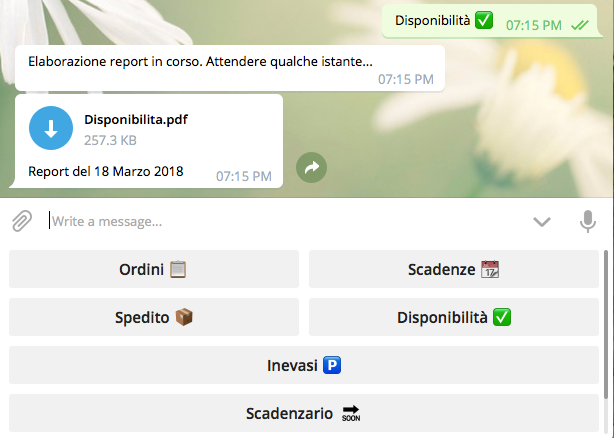
\includegraphics[scale=0.5]{screen/menu_disponibilita} 
    \caption{Menu Disponibilità}
     \end{center}
    Il bottone Disponibilità invece permette di scaricare direttamente il report di Disponibilità. Il report di disponibilità è profilato in base al tipo di utente, per cui la tabella che viene costruita in BI Service varia per utente. Lo stesso procedimento si ha anche per il bottone Inevasi. Lo scadenzario invece ha un altro livello innestato dove si può scegliere di scaricare il report totale di scadenze, quello scaduto oppure a scadere. Dal momento in cui il report viene scaricato è possibile visualizzarlo direttamente premendo un'altra volta sul nome del file senza evitando cosi di cercarlo nel file system del cellulare. Telegram gestisce diversi tipi di file di dimensione fino a 1.5GB e ciò permette di caricare anche file PDF di grandi dimensioni. 
\end{figure}  


\begin{figure}[h!]
   
    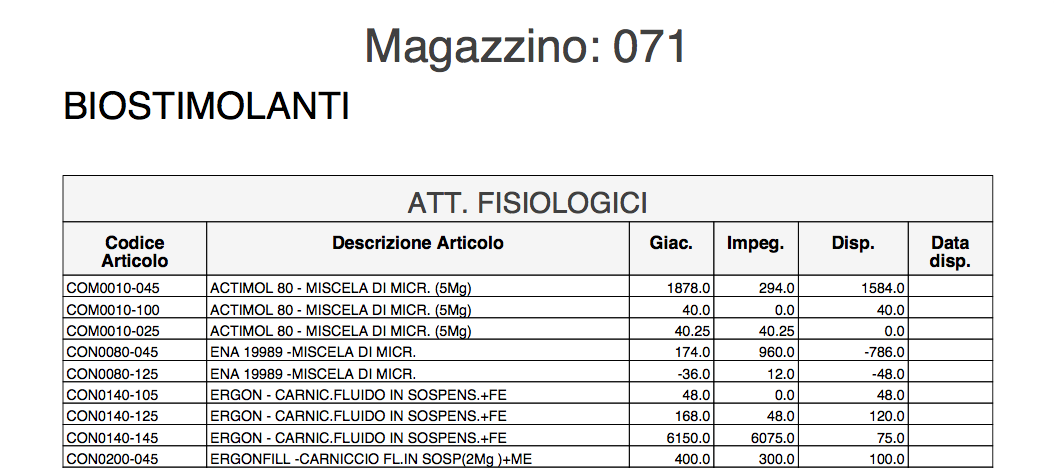
\includegraphics[scale=0.37]{screen/disponibilita} 
    \caption{Report Disponibilità}
     La figura 5.6 illustra una tabella che rappresenta la disponibilità giornaliera con il numero del magazzino e il codice identificativo dell’articolo in prima colonna.
\end{figure}  


\begin{figure}[h!]
   \begin{center}
   \textbf{Area amministrativa}\\
   \end{center}
   \begin{center}
    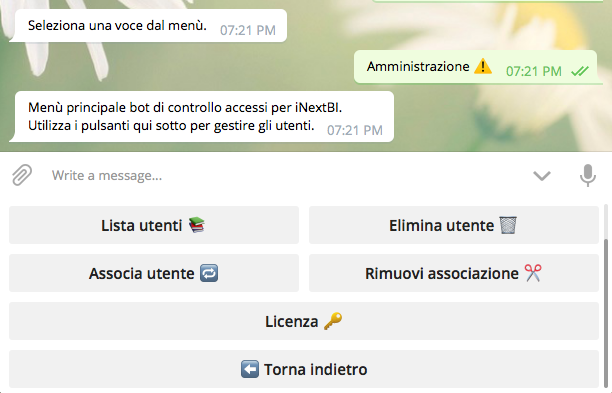
\includegraphics[scale=0.53]{screen/menu_admin} 
    \caption{Il menù di amministrazione}
    \end{center}
     Nella figura 5.7 vediamo invece come è composto il menù di amministrazione. In alto a sinistra troviamo la Lista utenti che visualizza sull'area della chat una lista degli utenti con i corrispondenti idTelegram che sono attualmente attivi e informazioni su eventuali associazioni con utenti B2B. In alto a destra invece il bottone Elimina utente permette di eliminare un utente non amministratore digitando semplicemente il suo idTelegram oppure il nome e cognome. 
\end{figure}  

\begin{figure}[h!]
   \begin{center}
   \textbf{Associazione utente B2B}\\
   \end{center}
   \begin{center}
    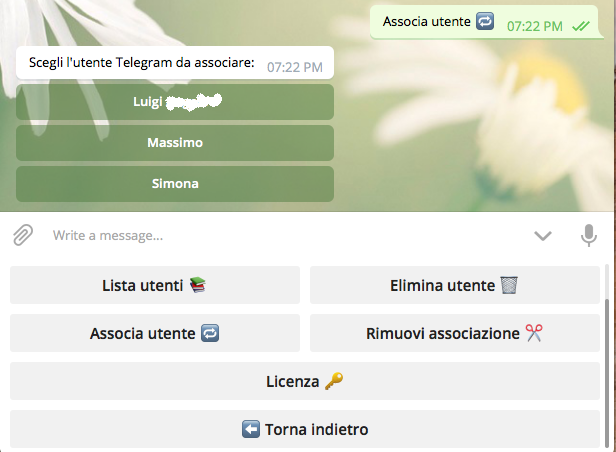
\includegraphics[scale=0.85]{screen/menu_associazione} 
    \caption{Associazione B2B}
    \end{center}
     Il menù di associazione utente permette di associare un id utente telegram con l'utente B2B facendo cosi in modo di avere un solo riferimento per utente. L'operazione di associazione avviene scegliendo prima un utente telegram da quelli che non risultano ancora associati. Per poter permettere all'utente amministratore di selezionare l'utente da associare è stata creata una tastiera inline con i nomi degli utenti. Premendo su un nome  si apre un'altra tastiera inline con le lettere dell'alfabeto. E’ sufficiente scegliere l'iniziale del nome dell'utente B2B per poterlo associare con quello di telegram.Per il bottone Rimuovi associazione invece abbiamo una sola lista di utenti associati rappresentati anche questi da un inline keyboard. Premendo su un nome, l'associazione utente telegram e utente B2B vine eliminata. 

\end{figure}  



\begin{figure}[h!]
   \begin{center}
   \textbf{Gestione Licenza}\\
   \end{center}
   \begin{center}
    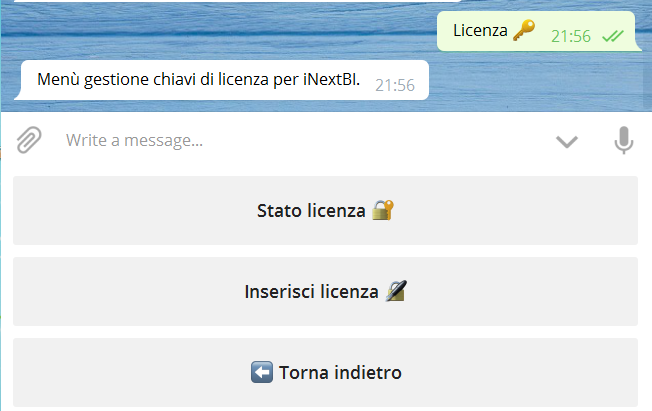
\includegraphics[scale=0.8]{screen/menu_licenza} 
    \caption{Licenze}
    \end{center}
   Per quanto riguarda il menù della licenza invece si hanno tre bottoni, il primo indica lo stato delle licenze per gli utenti generali, il secondo invece permette di inserire una licenza per gli utenti che si trovavano in stato di attesa. Dal momento che viene inserita una licenza valida, l'utente generico viene tolto dalla lista di attesa e può utilizzare le funzionalità dell'applicativo. Il terzo bottone invece permette di tornare al menù precedente.

\end{figure}  





